% ==================================================================
% hetmacro Codebook (LaTeX)
% Comprehensive documentation with theory, usage, and examples
% ==================================================================
\documentclass[12pt]{book}

% Style switch
\newif\ifmyoption
\myoptiontrue

% Core settings & fonts
\usepackage[T1]{fontenc}
\usepackage[sc]{mathpazo}
\usepackage{geometry}
\geometry{top=1in, bottom=1in, left=1in, right=1in}
\usepackage[Sonny]{fncychap}

% General utilities
\usepackage{url}
\usepackage{booktabs}
\usepackage{tabularx}
\usepackage{setspace}
\usepackage{csquotes}
\usepackage{enumitem}
\usepackage{xstring}
\usepackage{longtable}

% Mathematics
\usepackage{amsmath,amssymb,amsfonts,amsthm,mathtools}

% Code listings
\usepackage{listings}
\usepackage{xcolor}
\definecolor{codegreen}{rgb}{0,0.6,0}
\definecolor{codegray}{rgb}{0.5,0.5,0.5}
\definecolor{codepurple}{rgb}{0.58,0,0.82}
\definecolor{backcolour}{rgb}{0.95,0.95,0.92}

\lstdefinestyle{pythonstyle}{
    backgroundcolor=\color{backcolour},
    commentstyle=\color{codegreen},
    keywordstyle=\color{blue},
    numberstyle=\tiny\color{codegray},
    stringstyle=\color{codepurple},
    basicstyle=\ttfamily\small,
    breakatwhitespace=false,
    breaklines=true,
    captionpos=b,
    keepspaces=true,
    numbers=left,
    numbersep=5pt,
    showspaces=false,
    showstringspaces=false,
    showtabs=false,
    tabsize=2,
    frame=single,
    columns=fullflexible
}
\lstset{style=pythonstyle, language=Python}

% Hyperref
\usepackage[colorlinks=true,linkcolor=blue,urlcolor=blue,citecolor=blue]{hyperref}

% Custom environments
\newenvironment{functionbox}[1]{%
    \vspace{0.5em}
    \noindent\textbf{\texttt{#1}}\\[0.3em]
    \begin{tabular}{@{}p{0.95\textwidth}@{}}
}{%
    \end{tabular}
    \vspace{0.5em}
}

\newcommand{\argument}[3]{\texttt{#1} (\textit{#2}): #3}
\newcommand{\returns}[1]{\paragraph{Returns.} #1}
\newcommand{\connection}[1]{\paragraph{Connections.} #1}

% Argument list formatting (labels on their own line)
\newlist{arglist}{description}{1}
\setlist[arglist]{style=nextline,leftmargin=0pt,labelwidth=0pt,align=left,itemsep=0.2em}

% Replace bold labels with paragraph headings for consistent indentation
\let\oldtextbf\textbf
\newcommand{\labelpara}[1]{\paragraph{#1}\mbox{}\par\noindent\ignorespaces}
\newcommand{\formatlabel}[1]{%
    \IfStrEq{#1}{Purpose:}{\labelpara{Purpose.}}{%
    \IfStrEq{#1}{Arguments:}{\labelpara{Arguments.}}{%
    \IfStrEq{#1}{Example:}{\labelpara{Example.}}{%
    \IfStrEq{#1}{Workflow:}{\labelpara{Workflow.}}{%
    \IfStrEq{#1}{Algorithm:}{\labelpara{Algorithm.}}{%
    \IfStrEq{#1}{Note:}{\labelpara{Note.}}{%
    \IfStrEq{#1}{When to use:}{\labelpara{When to use.}}{%
    \oldtextbf{#1}}}}}}}}%
}
\renewcommand{\textbf}[1]{\formatlabel{#1}}

% Document metadata
\title{\vspace{-1cm}\textbf{hetmacro Codebook}\\[0.5em]\large A Comprehensive Guide to Numerical Tools\\for Heterogeneous Agent Macroeconomics}
\author{Rafael Lincoln \\ New York University}
\date{January 2026}

\begin{document}
\maketitle

\tableofcontents
\pagebreak

\begin{onehalfspacing}

% ==================================================================
\chapter{Introduction}
% ==================================================================

\section{Purpose and Philosophy}

The \texttt{hetmacro} package provides a self-contained, modular toolkit for solving structural macroeconomic models with heterogeneity. These models---including Aiyagari, Krusell-Smith, and HANK models---require agents to make optimal decisions over continuous state spaces, typically involving savings/consumption choices under idiosyncratic and aggregate uncertainty.

Solving such models numerically requires a carefully orchestrated pipeline:
\begin{enumerate}
    \item \textbf{Discretization}: Continuous state spaces must be approximated by grids; continuous stochastic processes (like income) must be discretized into Markov chains.
    \item \textbf{Backward Iteration}: Given prices, solve for optimal policy functions via dynamic programming (VFI, EGM).
    \item \textbf{Forward Iteration}: Given policies, compute the stationary distribution of agents across states.
    \item \textbf{Equilibrium}: Find prices that clear markets (e.g., asset supply equals capital demand).
    \item \textbf{Linearization}: For aggregate dynamics, compute sequence-space Jacobians.
\end{enumerate}

This codebook documents each module in \texttt{hetmacro}, explaining not just \emph{what} each function does, but \emph{why} it exists and \emph{how} it connects to other tools in the pipeline.

\section{Package Architecture}

The package is organized into two layers:

\subsection{Foundational Modules}
General-purpose numerical tools that can be used for any computational economics application:
\begin{itemize}
    \item \texttt{grids.py} -- State space discretization
    \item \texttt{quadrature.py} -- Numerical integration
    \item \texttt{interpolation.py} -- Function approximation
    \item \texttt{optimize.py} -- Root-finding and optimization
    \item \texttt{markov.py} -- Markov chain tools
    \item \texttt{utils.py} -- Economic primitives and utilities
\end{itemize}

\subsection{Heterogeneous Agent Tools}
Specialized routines for HA models:
\begin{itemize}
    \item \texttt{backward.py} -- Dynamic programming solvers
    \item \texttt{forward.py} -- Distribution iteration
    \item \texttt{steady\_state.py} -- Equilibrium solvers
    \item \texttt{ssj.py} -- Sequence-space Jacobians
    \item \texttt{dp\_tools.py}, \texttt{distributions.py} -- High-level wrappers
\end{itemize}

% ==================================================================
\chapter{Foundational Modules}
% ==================================================================

% ------------------------------------------------------------------
\section{\texttt{grids.py} -- State Space Discretization}
% ------------------------------------------------------------------

\subsection{Introduction and Economic Motivation}

In heterogeneous agent models, agents make decisions over continuous state variables---typically assets $a \in [\underline{a}, \bar{a}]$ and possibly other states like productivity, human capital, or housing. Since computers cannot store functions over continuous domains, we must discretize these spaces into finite grids.

The choice of grid matters substantially for accuracy and computational cost:
\begin{itemize}
    \item \textbf{Near borrowing constraints}: Policy functions often exhibit kinks near $a = \underline{a}$ where agents are constrained. Dense grid coverage here improves accuracy.
    \item \textbf{In the tail}: Wealthy agents' behavior matters less for aggregates but requires coverage for numerical stability.
    \item \textbf{Around specific values}: Some models have kinks at particular thresholds (e.g., tax brackets, collateral constraints).
\end{itemize}

This module provides flexible grid construction supporting various spacing strategies and the ability to concentrate points around specified locations.

\subsection{Core Class: \texttt{GridSpec}}

\begin{lstlisting}
@dataclass
class GridSpec:
    lower: float           # Lower bound of grid
    upper: float           # Upper bound of grid
    n_points: int          # Number of grid points
    spacing: str = "linear"          # Spacing method
    power: float = 1.0               # Exponent for power spacing
    concentration_points: Optional[Sequence[float]] = None
    concentration_weight: float = 0.0
    concentration_radius: Optional[float] = None
    custom_func: Optional[Callable] = None
\end{lstlisting}

\textbf{Purpose:} A specification object for one dimension of a grid. Use \texttt{GridSpec} when constructing multi-dimensional grids via \texttt{make\_grid\_nd}.

\textbf{Arguments:}
\begin{arglist}
    \item[\texttt{lower}] Lower bound of the state variable (e.g., borrowing limit $\underline{a}$).
    \item[\texttt{upper}] Upper bound (e.g., maximum asset level $\bar{a}$).
    \item[\texttt{n\_points}] Number of grid points. More points $\Rightarrow$ higher accuracy but slower computation.
    \item[\texttt{spacing}] One of \texttt{"linear"}, \texttt{"power"}, \texttt{"log"}, \texttt{"double\_exp"}, \texttt{"chebyshev"}, or \texttt{"custom"}.
    \item[\texttt{power}] For \texttt{spacing="power"}: exponent $\gamma$ where grid is $\underline{a} + (\bar{a}-\underline{a}) \cdot t^\gamma$ for $t \in [0,1]$. Values $>1$ concentrate points near lower bound.
    \item[\texttt{concentration\_points}] Sequence of values around which to concentrate grid points (e.g., kink locations).
    \item[\texttt{concentration\_weight}] Strength $\in [0,1]$ of concentration effect.
    \item[\texttt{concentration\_radius}] Scale parameter for concentration kernel. Defaults to 10\% of range.
    \item[\texttt{custom\_func}] For \texttt{spacing="custom"}: a function mapping $[0,1] \to [\text{lower}, \text{upper}]$.
\end{arglist}

\subsection{Function: \texttt{make\_grid\_1d}}

\begin{lstlisting}
def make_grid_1d(
    lower: float,
    upper: float,
    n: int,
    spacing: str = "linear",
    power: float = 1.0,
    concentration_points: Optional[Sequence[float]] = None,
    concentration_weight: float = 0.0,
    concentration_radius: Optional[float] = None,
    custom_func: Optional[Callable] = None,
) -> np.ndarray
\end{lstlisting}

\textbf{Purpose:} Create a one-dimensional grid with flexible spacing. This is the workhorse function for discretizing a single state variable.

\textbf{Arguments:}
\begin{arglist}
    \item[\texttt{lower, upper}] Bounds of the grid (inclusive). For assets, typically \texttt{lower=0} (or natural borrowing limit) and \texttt{upper} large enough to be non-binding.
    \item[\texttt{n}] Number of grid points (must be $\geq 2$).
    \item[\texttt{spacing}] Grid spacing method:
    \begin{itemize}
        \item \texttt{"linear"}: Equidistant points. Simple but inefficient near constraints.
        \item \texttt{"power"}: $a_i = \underline{a} + (\bar{a}-\underline{a})(i/(n-1))^\gamma$. Use $\gamma > 1$ to concentrate near $\underline{a}$.
        \item \texttt{"log"}: Logarithmically spaced. Requires \texttt{lower > 0}.
        \item \texttt{"double\_exp"}: Rognlie-style double exponential. Very dense near lower bound.
        \item \texttt{"chebyshev"}: Chebyshev nodes. Optimal for polynomial approximation.
        \item \texttt{"custom"}: User-provided transformation.
    \end{itemize}
    \item[\texttt{power}] Exponent for power spacing (default 1.0 = linear).
    \item[\texttt{concentration\_*}] Optional point concentration (see \texttt{GridSpec}).
    \item[\texttt{custom\_func}] Required if \texttt{spacing="custom"}.
\end{arglist}

\returns{1D NumPy array of grid points, sorted and with exact endpoints.}

\connection{Output feeds into \texttt{backward.py} for policy iteration, \texttt{interpolation.py} for function evaluation, and \texttt{forward.py} for distribution iteration.}

\textbf{Example:}
\begin{lstlisting}
import numpy as np
from hetmacro.grids import make_grid_1d

# Asset grid with power spacing (dense near borrowing constraint)
a_grid = make_grid_1d(
    lower=0.0, 
    upper=50.0, 
    n=200, 
    spacing="power", 
    power=2.0
)
print(f"First 5 points: {a_grid[:5]}")
# Dense near 0, sparse near 50

# Grid with concentration around kink at a=10
a_grid_kink = make_grid_1d(
    lower=0.0,
    upper=50.0,
    n=200,
    spacing="linear",
    concentration_points=[10.0],
    concentration_weight=0.5,
    concentration_radius=2.0
)
\end{lstlisting}

\subsection{Function: \texttt{make\_grid\_nd}}

\begin{lstlisting}
def make_grid_nd(
    specs: Sequence[GridSpec],
    cartesian: bool = False,
    tensor: bool = False,
    order: str = "C",
) -> Tuple[List[np.ndarray], Optional[np.ndarray]]
\end{lstlisting}

\textbf{Purpose:} Construct multi-dimensional grids from a list of \texttt{GridSpec} objects. Essential for models with multiple state variables (e.g., assets and human capital, or assets and housing).

\textbf{Arguments:}
\begin{arglist}
    \item[\texttt{specs}] Sequence of \texttt{GridSpec} objects, one per dimension.
    \item[\texttt{cartesian}] If \texttt{True}, also return the Cartesian product of all grids as a 2D array where each row is a state combination.
    \item[\texttt{tensor}] If \texttt{True}, return a tensor grid of shape $(n_1, n_2, \ldots, n_d, d)$.
    \item[\texttt{order}] Memory layout: \texttt{"C"} (row-major) or \texttt{"F"} (column-major, Fortran-style).
\end{arglist}

\returns{Tuple of (list of 1D grids, optional Cartesian/tensor grid).}

\connection{The 1D grids are used independently in \texttt{interpolation.py}; the Cartesian product is useful for computing expectations over joint distributions; the tensor grid is useful for reshaping policies over full state tensors.}

\textbf{Example:}
\begin{lstlisting}
from hetmacro.grids import GridSpec, make_grid_nd

# Two-dimensional grid: assets and human capital
specs = [
    GridSpec(lower=0, upper=50, n_points=100, spacing="power", power=2),
    GridSpec(lower=0.5, upper=2.0, n_points=20, spacing="linear"),
]
grids, product = make_grid_nd(specs, cartesian=True)
a_grid, h_grid = grids
print(f"Asset grid: {len(a_grid)} points")
print(f"Human capital grid: {len(h_grid)} points")
print(f"State space: {product.shape[0]} total states")

# Tensor grid with shape (n_a, n_h, 2)
grids, tensor = make_grid_nd(specs, tensor=True)
print(tensor.shape)
\end{lstlisting}

\subsection{Function: \texttt{make\_asset\_grid}}

\begin{lstlisting}
def make_asset_grid(
    amin: float,
    amax: float,
    n: int,
    curvature: float = 2.0,
) -> np.ndarray
\end{lstlisting}

\textbf{Purpose:} Convenience function for the common case of an asset grid with power spacing. This is a thin wrapper around \texttt{make\_grid\_1d} with sensible defaults for incomplete markets models.

\textbf{Arguments:}
\begin{arglist}
    \item[\texttt{amin}] Borrowing limit (often 0 or natural borrowing limit).
    \item[\texttt{amax}] Upper bound on assets.
    \item[\texttt{n}] Number of grid points.
    \item[\texttt{curvature}] Power exponent (default 2.0 works well in practice).
\end{arglist}

\returns{1D array of asset grid points.}

\textbf{Example:}
\begin{lstlisting}
from hetmacro.grids import make_asset_grid

# Standard Aiyagari-style asset grid
a_grid = make_asset_grid(amin=0, amax=50, n=500, curvature=2.0)
\end{lstlisting}

\subsection{Function: \texttt{double\_exponential\_grid}}

\begin{lstlisting}
def double_exponential_grid(amin: float, amax: float, n: int) -> np.ndarray
\end{lstlisting}

\textbf{Purpose:} Rognlie-style double exponential grid, which provides extremely dense coverage near the lower bound. Useful when policy functions have sharp features near constraints.

\textbf{Mathematical form:} Let $\bar{u} = \log(1 + \log(1 + a_{\max} - a_{\min}))$. The grid is:
\[
a_i = a_{\min} + \exp(\exp(u_i) - 1) - 1, \quad u_i \in \text{linspace}(0, \bar{u}, n)
\]

\subsection{Function: \texttt{cartesian\_product} / \texttt{gridmake}}

\begin{lstlisting}
def cartesian_product(*grids, order: str = "C") -> np.ndarray
def gridmake(*grids, order: str = "C") -> np.ndarray  # alias
\end{lstlisting}

\textbf{Purpose:} Compute the Cartesian product of multiple 1D grids. Each row of the output represents one combination of state values.

\textbf{Arguments:}
\begin{arglist}
    \item[\texttt{*grids}] Variable number of 1D arrays.
    \item[\texttt{order}] Memory layout for iteration order.
\end{arglist}

\returns{2D array of shape $(n_1 \times n_2 \times \cdots, d)$ where $d$ is the number of grids.}

\textbf{Example:}
\begin{lstlisting}
from hetmacro.grids import cartesian_product
import numpy as np

a_grid = np.array([0, 1, 2])
e_grid = np.array([0.5, 1.0, 1.5])
states = cartesian_product(a_grid, e_grid)
# states[0] = [0, 0.5], states[1] = [0, 1.0], etc.
\end{lstlisting}

\subsection{Function: \texttt{tensor\_product}}

\begin{lstlisting}
def tensor_product(*grids) -> np.ndarray
\end{lstlisting}

\textbf{Purpose:} Construct a tensor grid that preserves the full $n_1 \times \cdots \times n_d$ structure, with the last axis storing coordinates.

\textbf{Arguments:}
\begin{arglist}
    \item[\texttt{*grids}] Variable number of 1D arrays.
\end{arglist}

\returns{Array of shape $(n_1, n_2, \ldots, n_d, d)$.}

\textbf{Example:}
\begin{lstlisting}
from hetmacro.grids import tensor_product
import numpy as np

a_grid = np.array([0, 1, 2])
e_grid = np.array([0.5, 1.0])
tensor = tensor_product(a_grid, e_grid)
# tensor.shape == (3, 2, 2)
\end{lstlisting}

\subsection{Function: \texttt{smolyak\_sparse\_grid}}

\begin{lstlisting}
def smolyak_sparse_grid(
    specs: Sequence[GridSpec],
    level: int,
    rule: str = "clenshaw_curtis",
    unique_decimals: int = 14,
) -> np.ndarray
\end{lstlisting}

\textbf{Purpose:} Construct a Smolyak sparse grid on a hyper-rectangle using nested Clenshaw--Curtis nodes to reduce the curse of dimensionality.

\textbf{Arguments:}
\begin{arglist}
    \item[\texttt{specs}] GridSpec list; uses only \texttt{lower} and \texttt{upper} per dimension.
    \item[\texttt{level}] Smolyak level ($\geq 1$). Higher levels add more points.
    \item[\texttt{rule}] 1D nested rule (currently \texttt{"clenshaw\_curtis"}).
    \item[\texttt{unique\_decimals}] Decimal rounding for deduplication of nested nodes.
\end{arglist}

\returns{Array of unique sparse-grid points of shape $(n_{\text{points}}, d)$.}

\textbf{Example:}
\begin{lstlisting}
from hetmacro.grids import GridSpec, smolyak_sparse_grid

specs = [
    GridSpec(lower=-1, upper=1, n_points=0),
    GridSpec(lower=-1, upper=1, n_points=0),
]
points = smolyak_sparse_grid(specs, level=3)
print(points.shape)
\end{lstlisting}

% ------------------------------------------------------------------
\section{\texttt{quadrature.py} -- Numerical Integration}
% ------------------------------------------------------------------

\subsection{Introduction and Economic Motivation}

Expectations are fundamental in dynamic economics. Agents form expectations over future states:
\[
\mathbb{E}[V(a', e') \mid e] = \int V(a', e') \, dF(e' \mid e)
\]
When shocks are continuous (e.g., normally distributed innovations), we cannot sum over states---we must integrate. Quadrature rules approximate integrals using weighted sums:
\[
\int f(x) w(x) \, dx \approx \sum_{i=1}^{n} w_i f(x_i)
\]
where $\{x_i\}$ are nodes and $\{w_i\}$ are weights chosen to make the approximation exact for polynomials up to some degree.

\textbf{Key insight:} Different distributions require different quadrature rules. Gauss-Hermite is optimal for normally distributed shocks; Gauss-Legendre for bounded uniform distributions.

\subsubsection{Theory: Gaussian Quadrature}

Gaussian quadrature is a family of methods for approximating integrals of the form:
\[
\int_a^b f(x) \, w(x) \, dx \approx \sum_{i=1}^{n} w_i \, f(x_i)
\]
where $w(x)$ is a \textbf{weighting function} (not to be confused with the quadrature weights $w_i$).

The key insight is that if the nodes $\{x_i\}$ are chosen as the roots of orthogonal polynomials associated with $w(x)$, then the approximation is \textbf{exact for polynomials of degree up to $2n-1$}. This is twice as accurate as methods with equally-spaced nodes (like Simpson or Trapezoidal rules).

Each quadrature rule in this module corresponds to a specific weighting function and its associated orthogonal polynomials:

\begin{center}
\begin{tabular}{llll}
\toprule
\textbf{Function} & \textbf{Weight function $w(x)$} & \textbf{Domain} & \textbf{Orthogonal Polynomial} \\
\midrule
\texttt{qnwlege} & $1$ (uniform) & $[a, b]$ & Legendre \\
\texttt{qnwcheb} & $1/\sqrt{1-x^2}$ & $[-1, 1]$ & Chebyshev \\
\texttt{qnwnorm} & $e^{-x^2}$ (Gaussian) & $(-\infty, \infty)$ & Hermite \\
\texttt{qnwbeta} & $x^{a-1}(1-x)^{b-1}$ & $[0, 1]$ & Jacobi \\
\texttt{qnwgamma} & $x^{a-1}e^{-x}$ & $[0, \infty)$ & Laguerre \\
\bottomrule
\end{tabular}
\end{center}

\paragraph{Why different rules?} Each rule places nodes where the weight function $w(x)$ concentrates probability mass:
\begin{itemize}
    \item \textbf{Gauss-Hermite} (\texttt{qnwnorm}): Nodes cluster around the mean. Optimal for normal distributions---the workhorse for computing expectations over income shocks.
    \item \textbf{Gauss-Legendre} (\texttt{qnwlege}): Nodes spread across the interval with slight concentration at endpoints. Best for smooth functions on bounded intervals.
    \item \textbf{Gauss-Chebyshev} (\texttt{qnwcheb}): Nodes are Chebyshev points (cosines of equally-spaced angles). Optimal for polynomial interpolation and avoids Runge's phenomenon.
    \item \textbf{Gauss-Jacobi} (\texttt{qnwbeta}): Handles Beta distributions on $[0,1]$.
    \item \textbf{Gauss-Laguerre} (\texttt{qnwgamma}): For Gamma distributions with positive support.
\end{itemize}

\paragraph{Convenience wrappers.} Some functions adapt the basic rules for common use cases:
\begin{itemize}
    \item \texttt{qnwlogn}: Transforms Hermite nodes via exponentiation for lognormal distributions.
    \item \texttt{qnwunif}: Adapts Legendre and normalizes weights for uniform density.
    \item \texttt{qnwnorm\_mv}: Tensor product of Hermite rules for multivariate normal.
\end{itemize}

\paragraph{Non-Gaussian rules.} The functions \texttt{qnwsimp} (Simpson) and \texttt{qnwtrap} (Trapezoidal) are \textbf{Newton-Cotes} quadrature, which use equally-spaced nodes. These are simpler but less accurate for smooth functions. Use them when function values are only available on a pre-specified grid.

\subsection{Function: \texttt{qnwlege}}

\begin{lstlisting}
def qnwlege(n: int, a: float, b: float) -> Tuple[np.ndarray, np.ndarray]
\end{lstlisting}

\textbf{Purpose:} Gauss-Legendre quadrature for integrals over bounded intervals $[a, b]$. The weighting function is $w(x) = 1$ (uniform), so this approximates:
\[
\int_a^b f(x) \, dx \approx \sum_{i=1}^{n} w_i \, f(x_i)
\]

\textbf{Arguments:}
\begin{arglist}
    \item[\texttt{n}] Number of nodes. With $n$ nodes, polynomials of degree $\leq 2n-1$ are integrated exactly.
    \item[\texttt{a, b}] Integration bounds.
\end{arglist}

\returns{Tuple \texttt{(nodes, weights)} for approximating $\int_a^b f(x) dx$.}

\textbf{When to use:} General-purpose integration on bounded intervals. Optimal for smooth functions.

\subsection{Function: \texttt{qnwcheb}}

\begin{lstlisting}
def qnwcheb(n: int, a: float, b: float) -> Tuple[np.ndarray, np.ndarray]
\end{lstlisting}

\textbf{Purpose:} Gauss-Chebyshev quadrature with weighting function $w(x) = 1/\sqrt{1-x^2}$. Approximates:
\[
\int_a^b \frac{f(x)}{\sqrt{1-x^2}} \, dx \approx \sum_{i=1}^{n} w_i \, f(x_i)
\]
where $x$ is scaled from $[a,b]$ to $[-1,1]$.

\textbf{Arguments:}
\begin{arglist}
    \item[\texttt{n}] Number of nodes (Chebyshev points).
    \item[\texttt{a, b}] Integration bounds (mapped to $[-1,1]$).
\end{arglist}

\returns{Tuple \texttt{(nodes, weights)}.}

\textbf{When to use:} 
\begin{itemize}
    \item When constructing Chebyshev polynomial approximations (nodes are optimal interpolation points).
    \item For integrals with weight function $1/\sqrt{1-x^2}$.
    \item When you want to avoid Runge's phenomenon in polynomial interpolation.
\end{itemize}

\textbf{Special property:} The Chebyshev nodes are $x_i = \cos\left(\frac{2i-1}{2n}\pi\right)$ for $i=1,\ldots,n$, which are cosines of equally-spaced angles.

\subsection{Function: \texttt{qnwnorm}}

\begin{lstlisting}
def qnwnorm(
    n: int, 
    mu: float = 0.0, 
    sigma: float = 1.0
) -> Tuple[np.ndarray, np.ndarray]
\end{lstlisting}

\textbf{Purpose:} Gauss-Hermite quadrature for computing expectations under normal distributions. This is the most commonly used quadrature in macro for approximating:
\[
\mathbb{E}[f(X)] \text{ where } X \sim \mathcal{N}(\mu, \sigma^2)
\]

\textbf{Arguments:}
\begin{arglist}
    \item[\texttt{n}] Number of quadrature nodes. Higher $n$ = more accurate but more expensive. Typically 5-9 is sufficient.
    \item[\texttt{mu}] Mean of the normal distribution.
    \item[\texttt{sigma}] Standard deviation.
\end{arglist}

\returns{Tuple \texttt{(nodes, weights)} where \texttt{nodes} are evaluation points and \texttt{weights} sum to 1.}

\connection{Used in \texttt{markov.py} for discretizing AR(1) processes; can be used directly for computing expectations in models with continuous shocks.}

\textbf{Example:}
\begin{lstlisting}
from hetmacro.quadrature import qnwnorm
import numpy as np

# Approximate E[exp(X)] where X ~ N(0, 0.1^2)
# True answer: exp(0.5 * 0.1^2) = 1.00501
nodes, weights = qnwnorm(n=5, mu=0.0, sigma=0.1)
approx = np.dot(weights, np.exp(nodes))
print(f"Approximation: {approx:.5f}")  # Very close to 1.00501
\end{lstlisting}

\subsection{Function: \texttt{qnwlogn}}

\begin{lstlisting}
def qnwlogn(
    n: int, 
    mu: float = 0.0, 
    sigma: float = 1.0
) -> Tuple[np.ndarray, np.ndarray]
\end{lstlisting}

\textbf{Purpose:} Quadrature for lognormal distributions. If $\log X \sim \mathcal{N}(\mu, \sigma^2)$, this provides nodes and weights for $\mathbb{E}[f(X)]$.

\textbf{Note:} The nodes are exponentiated Gauss-Hermite nodes; weights remain the same.

\subsection{Function: \texttt{qnwunif}}

\begin{lstlisting}
def qnwunif(n: int, a: float, b: float) -> Tuple[np.ndarray, np.ndarray]
\end{lstlisting}

\textbf{Purpose:} Quadrature for uniform distribution on $[a, b]$. Weights are normalized so $\sum w_i = 1$.

\subsection{Function: \texttt{qnwbeta}}

\begin{lstlisting}
def qnwbeta(n: int, a: float = 1.0, b: float = 1.0) -> Tuple[np.ndarray, np.ndarray]
\end{lstlisting}

\textbf{Purpose:} Quadrature for Beta$(a, b)$ distribution on $[0, 1]$. Useful for modeling bounded random variables like labor supply elasticities or preference heterogeneity.

\subsection{Function: \texttt{qnwgamma}}

\begin{lstlisting}
def qnwgamma(n: int, a: float = 1.0, b: float = 1.0) -> Tuple[np.ndarray, np.ndarray]
\end{lstlisting}

\textbf{Purpose:} Quadrature for Gamma$(a, b)$ distribution (shape $a$, scale $b$). Useful for modeling income distributions or shock processes with positive support.

\subsection{Function: \texttt{qnwnorm\_mv}}

\begin{lstlisting}
def qnwnorm_mv(
    n: np.ndarray, 
    mu: np.ndarray, 
    Sigma: np.ndarray
) -> Tuple[np.ndarray, np.ndarray]
\end{lstlisting}

\textbf{Purpose:} Multivariate normal quadrature via tensor product. For $X \sim \mathcal{N}(\mu, \Sigma)$, computes nodes and weights for $\mathbb{E}[f(X)]$.

\textbf{Arguments:}
\begin{arglist}
    \item[\texttt{n}] Array of number of nodes per dimension.
    \item[\texttt{mu}] Mean vector.
    \item[\texttt{Sigma}] Covariance matrix (must be positive definite).
\end{arglist}

\returns{Tuple \texttt{(nodes, weights)} where \texttt{nodes} has shape $(n_1 \times \cdots \times n_d, d)$.}

\textbf{Example:}
\begin{lstlisting}
from hetmacro.quadrature import qnwnorm_mv
import numpy as np

# Bivariate normal with correlation
mu = np.array([0.0, 0.0])
Sigma = np.array([[1.0, 0.5], [0.5, 1.0]])
nodes, weights = qnwnorm_mv(n=np.array([5, 5]), mu=mu, Sigma=Sigma)
print(f"Number of quadrature points: {len(weights)}")  # 25
\end{lstlisting}

\subsection{Functions: \texttt{qnwsimp}, \texttt{qnwtrap}}

\begin{lstlisting}
def qnwsimp(n: int, a: float, b: float) -> Tuple[np.ndarray, np.ndarray]
def qnwtrap(n: int, a: float, b: float) -> Tuple[np.ndarray, np.ndarray]
\end{lstlisting}

\textbf{Purpose:} Newton-Cotes rules (Simpson's and Trapezoidal) for numerical integration. These use equally-spaced nodes and are simpler but less accurate than Gaussian quadrature for smooth functions.

\textbf{When to use:} When function values are only available on a pre-specified grid (e.g., integrating over a distribution that's already on an asset grid).

% ------------------------------------------------------------------
\section{\texttt{interpolation.py} -- Function Approximation}
% ------------------------------------------------------------------

\subsection{Introduction and Economic Motivation}

In dynamic programming, we iterate on functions defined on grids. However, optimal policies often require evaluating functions at off-grid points. For example, in the Endogenous Grid Method (EGM), we compute:
\[
c^*(a, e) = c_{\text{endog}}(a^{\text{endog}}(a, e))
\]
where $a^{\text{endog}}$ may not lie on the asset grid. Interpolation fills this gap.

Additionally, for computing stationary distributions with continuous policies, we need the ``lottery'' method: given a policy $a'(a, e)$ that falls between grid points $a_i < a' < a_{i+1}$, we split the mass probabilistically.

\subsection{Function: \texttt{interp\_linear}}

\begin{lstlisting}
def interp_linear(
    x_grid: np.ndarray, 
    y: np.ndarray, 
    x_new: np.ndarray
) -> np.ndarray
\end{lstlisting}

\textbf{Purpose:} Vectorized 1D linear interpolation. Given function values $y = f(x_{\text{grid}})$, evaluate at new points $x_{\text{new}}$.

\textbf{Arguments:}
\begin{arglist}
    \item[\texttt{x\_grid}] 1D array of grid points (must be sorted ascending).
    \item[\texttt{y}] Function values. Shape \texttt{(n,)} for single function or \texttt{(m, n)} for $m$ functions on the same grid.
    \item[\texttt{x\_new}] Points at which to interpolate.
\end{arglist}

\returns{Interpolated values, same shape as \texttt{x\_new} (or \texttt{(m,) + x\_new.shape} for multiple functions).}

\connection{Core building block for EGM (\texttt{backward.py}). Also used in \texttt{get\_lottery} for distribution iteration.}

\textbf{Example:}
\begin{lstlisting}
from hetmacro.interpolation import interp_linear
import numpy as np

# Interpolate consumption policy at off-grid asset values
a_grid = np.linspace(0, 10, 100)
c_policy = 0.05 * a_grid + 1.0  # Example: linear consumption
a_new = np.array([2.5, 5.5, 7.3])
c_new = interp_linear(a_grid, c_policy, a_new)
\end{lstlisting}

\subsection{Function: \texttt{interp\_bilinear}}

\begin{lstlisting}
def interp_bilinear(
    x_grid: np.ndarray,
    y_grid: np.ndarray,
    z: np.ndarray,
    x_new: np.ndarray,
    y_new: np.ndarray,
) -> np.ndarray
\end{lstlisting}

\textbf{Purpose:} Bilinear interpolation on a 2D rectilinear grid. For functions of two state variables $f(x, y)$.

\textbf{Arguments:}
\begin{arglist}
    \item[\texttt{x\_grid, y\_grid}] 1D arrays defining the grid in each dimension.
    \item[\texttt{z}] Function values, shape \texttt{(len(y\_grid), len(x\_grid))}.
    \item[\texttt{x\_new, y\_new}] Points at which to interpolate.
\end{arglist}

\returns{Interpolated values at \texttt{(x\_new, y\_new)} pairs.}

\subsection{Function: \texttt{get\_lottery}}

\begin{lstlisting}
def get_lottery(
    a_policy: np.ndarray, 
    a_grid: np.ndarray
) -> Tuple[np.ndarray, np.ndarray]
\end{lstlisting}

\textbf{Purpose:} Compute lottery indices and probabilities for distribution iteration. When agents choose $a' \in (a_i, a_{i+1})$, we assign probability $\pi_i$ to $a_i$ and $1 - \pi_i$ to $a_{i+1}$, where:
\[
\pi_i = \frac{a_{i+1} - a'}{a_{i+1} - a_i}
\]

\textbf{Arguments:}
\begin{arglist}
    \item[\texttt{a\_policy}] Policy function values (any shape).
    \item[\texttt{a\_grid}] Asset grid (1D, sorted).
\end{arglist}

\returns{Tuple \texttt{(a\_i, a\_pi)} where \texttt{a\_i} is the lower grid index and \texttt{a\_pi} is the probability on \texttt{a\_i}.}

\connection{Essential input to \texttt{forward\_iteration} in \texttt{forward.py}. The ``lottery'' method is how we iterate distributions forward when policies are continuous.}

\textbf{Example:}
\begin{lstlisting}
from hetmacro.interpolation import get_lottery
import numpy as np

a_grid = np.array([0, 1, 2, 3, 4])
a_policy = np.array([0.5, 1.7, 2.3])  # Off-grid choices

a_i, a_pi = get_lottery(a_policy, a_grid)
# a_i = [0, 1, 2] -- lower indices
# a_pi = [0.5, 0.3, 0.7] -- probabilities on lower point
\end{lstlisting}

\subsection{Chebyshev Approximation Functions}

\begin{lstlisting}
def cheb_nodes(n: int, a: float, b: float) -> np.ndarray
def cheb_basis(x: np.ndarray, n: int, a: float, b: float) -> np.ndarray
def cheb_coef(f: Callable, n: int, a: float, b: float) -> np.ndarray
def cheb_eval(coef: np.ndarray, x: np.ndarray, a: float, b: float) -> np.ndarray
\end{lstlisting}

\textbf{Purpose:} Chebyshev polynomial approximation provides highly accurate function representation with minimal oscillation (Runge phenomenon avoidance).

\textbf{Workflow:}
\begin{enumerate}
    \item Generate Chebyshev nodes with \texttt{cheb\_nodes}
    \item Fit coefficients with \texttt{cheb\_coef} given a function
    \item Evaluate approximation at arbitrary points with \texttt{cheb\_eval}
\end{enumerate}

\textbf{Example:}
\begin{lstlisting}
from hetmacro.interpolation import cheb_coef, cheb_eval
import numpy as np

# Approximate exp(x) on [-1, 1]
coef = cheb_coef(np.exp, n=10, a=-1, b=1)
x_test = np.linspace(-1, 1, 100)
approx = cheb_eval(coef, x_test, a=-1, b=1)
error = np.max(np.abs(approx - np.exp(x_test)))
print(f"Max error: {error:.2e}")  # Very small
\end{lstlisting}

\subsection{Spline Functions}

\begin{lstlisting}
def spline_coef(x: np.ndarray, y: np.ndarray, kind: str = "cubic")
def spline_eval(coef, x_new: np.ndarray) -> np.ndarray
\end{lstlisting}

\textbf{Purpose:} Cubic spline interpolation for smooth function approximation. Returns a SciPy spline object.

% ------------------------------------------------------------------
\section{\texttt{optimize.py} -- Root-Finding and Optimization}
% ------------------------------------------------------------------

\subsection{Introduction and Economic Motivation}

Equilibrium in economic models often requires finding roots of excess demand functions or optimizing objective functions. For example:
\begin{itemize}
    \item \textbf{Market clearing}: Find interest rate $r^*$ such that $A(r^*) - K(r^*) = 0$.
    \item \textbf{Optimal policy}: Find consumption $c^*$ maximizing $u(c) + \beta \mathbb{E}[V(a', e')]$.
\end{itemize}

This module wraps SciPy's optimization routines with a consistent API and sensible defaults.

\subsection{Root-Finding Functions}

\subsubsection{\texttt{bisect}}
\begin{lstlisting}
def bisect(
    f: Callable, 
    a: float, 
    b: float, 
    args=(), 
    tol: float = 1e-12, 
    max_iter: int = 100
) -> float
\end{lstlisting}

\textbf{Purpose:} Bisection method for finding roots. Guaranteed to converge if $f(a)$ and $f(b)$ have opposite signs.

\textbf{When to use:} For well-behaved monotonic functions like excess demand for capital. Simple and robust.

\subsubsection{\texttt{brentq}}
\begin{lstlisting}
def brentq(
    f: Callable, 
    a: float, 
    b: float, 
    args=(), 
    tol: float = 1e-12
) -> float
\end{lstlisting}

\textbf{Purpose:} Brent's method---combines bisection with inverse quadratic interpolation. Faster than bisection while retaining guaranteed convergence.

\textbf{When to use:} Default choice for 1D root-finding with bracketed roots.

\subsubsection{\texttt{newton}}
\begin{lstlisting}
def newton(
    f: Callable,
    x0: float,
    fprime: Callable,
    args=(),
    tol: float = 1e-8,
    max_iter: int = 50,
) -> float
\end{lstlisting}

\textbf{Purpose:} Newton-Raphson method using derivative information. Quadratic convergence near root.

\textbf{When to use:} When you have an analytical derivative and need fast convergence.

\subsubsection{\texttt{secant}}
\begin{lstlisting}
def secant(
    f: Callable, 
    x0: float, 
    args=(), 
    tol: float = 1e-8, 
    max_iter: int = 50
) -> float
\end{lstlisting}

\textbf{Purpose:} Secant method---derivative-free approximation of Newton's method.

\subsubsection{\texttt{broyden}}
\begin{lstlisting}
def broyden(
    f: Callable, 
    x0: np.ndarray, 
    args=(), 
    tol: float = 1e-8
) -> np.ndarray
\end{lstlisting}

\textbf{Purpose:} Broyden's method for systems of nonlinear equations $F(x) = 0$.

\textbf{When to use:} Multi-dimensional root-finding (e.g., joint market clearing in multiple markets).

\subsection{Optimization Functions}

\subsubsection{\texttt{golden\_search}}
\begin{lstlisting}
def golden_search(
    f: Callable, 
    a: float, 
    b: float, 
    args=(), 
    tol: float = 1e-8
) -> float
\end{lstlisting}

\textbf{Purpose:} Golden section search for 1D minimization on a bounded interval.

\textbf{When to use:} Minimizing unimodal functions when derivative is unavailable.

\subsubsection{\texttt{brent\_min}}
\begin{lstlisting}
def brent_min(
    f: Callable, 
    a: float, 
    b: float, 
    args=(), 
    tol: float = 1e-8
) -> float
\end{lstlisting}

\textbf{Purpose:} Brent's method for 1D minimization. Generally faster than golden section.

\subsubsection{\texttt{nelder\_mead}}
\begin{lstlisting}
def nelder_mead(
    f: Callable, 
    x0: np.ndarray, 
    args=(), 
    tol: float = 1e-8
) -> Tuple[np.ndarray, float]
\end{lstlisting}

\textbf{Purpose:} Nelder-Mead simplex algorithm for derivative-free multi-dimensional optimization.

\returns{Tuple \texttt{(x\_opt, f\_opt)} of optimal point and function value.}

\textbf{Example:}
\begin{lstlisting}
from hetmacro.optimize import bisect, brentq

# Find equilibrium interest rate
def excess_demand(r, A_supply_func, K_demand_func):
    return A_supply_func(r) - K_demand_func(r)

r_star = brentq(excess_demand, a=0.01, b=0.05, 
                args=(A_supply, K_demand))
\end{lstlisting}

% ------------------------------------------------------------------
\section{\texttt{markov.py} -- Markov Chain Tools}
% ------------------------------------------------------------------

\subsection{Introduction and Economic Motivation}

Many economic models feature persistent idiosyncratic shocks, typically modeled as AR(1) processes:
\[
\log e_{t+1} = \rho \log e_t + \sigma \varepsilon_{t+1}, \quad \varepsilon_t \sim \mathcal{N}(0, 1)
\]
For numerical solution, we discretize this continuous process into a finite-state Markov chain with states $\{e_1, \ldots, e_n\}$ and transition matrix $\Pi$ where $\Pi_{ij} = \Pr(e_{t+1} = e_j \mid e_t = e_i)$.

Two main methods exist: \textbf{Tauchen} (older, based on CDF matching) and \textbf{Rouwenhorst} (more accurate for highly persistent processes).

\subsection{Function: \texttt{rouwenhorst}}

\begin{lstlisting}
def rouwenhorst(
    n: int, 
    rho: float, 
    sigma: float, 
    mu: float = 0.0
) -> Tuple[np.ndarray, np.ndarray]
\end{lstlisting}

\textbf{Purpose:} Rouwenhorst discretization of AR(1) process. Preferred method for highly persistent processes ($\rho > 0.9$).

\textbf{Arguments:}
\begin{arglist}
    \item[\texttt{n}] Number of states (typically 5-11).
    \item[\texttt{rho}] Persistence parameter of AR(1).
    \item[\texttt{sigma}] Standard deviation of innovation $\varepsilon_t$.
    \item[\texttt{mu}] Unconditional mean (default 0).
\end{arglist}

\returns{Tuple \texttt{(states, Pi)} where \texttt{states} is 1D array of state values and \texttt{Pi} is $n \times n$ transition matrix.}

\connection{Output feeds directly into \texttt{backward.py} for computing conditional expectations in Bellman equations.}

\textbf{Example:}
\begin{lstlisting}
from hetmacro.markov import rouwenhorst, stationary_distribution

# Discretize typical income process
rho, sigma = 0.95, 0.1
e_states, Pi = rouwenhorst(n=7, rho=rho, sigma=sigma)

# Compute stationary distribution
pi = stationary_distribution(Pi)
print(f"States: {e_states}")
print(f"Stationary probabilities: {pi}")
\end{lstlisting}

\subsection{Function: \texttt{tauchen}}

\begin{lstlisting}
def tauchen(
    n: int,
    rho: float,
    sigma: float,
    mu: float = 0.0,
    n_std: float = 3.0,
) -> Tuple[np.ndarray, np.ndarray]
\end{lstlisting}

\textbf{Purpose:} Tauchen method for AR(1) discretization. Uses equally-spaced states covering $\pm n_{\text{std}}$ standard deviations.

\textbf{Arguments:}
\begin{arglist}
    \item[\texttt{n}] Number of states.
    \item[\texttt{rho}] Persistence.
    \item[\texttt{sigma}] Innovation standard deviation.
    \item[\texttt{mu}] Unconditional mean.
    \item[\texttt{n\_std}] Number of standard deviations to cover (default 3).
\end{arglist}

\textbf{When to use:} For less persistent processes ($\rho < 0.9$); Rouwenhorst is generally preferred otherwise.

\subsection{Function: \texttt{stationary\_distribution}}

\begin{lstlisting}
def stationary_distribution(
    P: np.ndarray, 
    method: str = "eigen", 
    tol: float = 1e-12
) -> np.ndarray
\end{lstlisting}

\textbf{Purpose:} Compute the stationary distribution $\pi$ satisfying $\pi = \Pi' \pi$.

\textbf{Arguments:}
\begin{arglist}
    \item[\texttt{P}] Transition matrix (rows sum to 1).
    \item[\texttt{method}] Either \texttt{"eigen"} (find unit eigenvalue) or \texttt{"iterate"} (power iteration).
    \item[\texttt{tol}] Convergence tolerance for iteration method.
\end{arglist}

\returns{1D array of stationary probabilities summing to 1.}

\subsection{Function: \texttt{simulate\_markov}}

\begin{lstlisting}
def simulate_markov(
    P: np.ndarray, 
    s0: int, 
    T: int, 
    random_state=None
) -> np.ndarray
\end{lstlisting}

\textbf{Purpose:} Simulate a sample path of Markov chain indices.

\textbf{Arguments:}
\begin{arglist}
    \item[\texttt{P}] Transition matrix.
    \item[\texttt{s0}] Initial state index.
    \item[\texttt{T}] Number of periods to simulate.
    \item[\texttt{random\_state}] Seed for reproducibility.
\end{arglist}

\returns{1D integer array of state indices over time.}

% ------------------------------------------------------------------
\section{\texttt{utils.py} -- Economic Primitives and Utilities}
% ------------------------------------------------------------------

\subsection{Introduction}

This module provides commonly-used economic functions (CRRA utility, CES aggregator) and general numerical utilities (fixed-point iteration, numerical differentiation, timing).

\subsection{Utility Functions}

\subsubsection{\texttt{crra\_utility}}
\begin{lstlisting}
def crra_utility(c: np.ndarray, gamma: float) -> np.ndarray
\end{lstlisting}

\textbf{Purpose:} Constant Relative Risk Aversion utility:
\[
u(c) = \begin{cases} \frac{c^{1-\gamma}}{1-\gamma} & \gamma \neq 1 \\ \log(c) & \gamma = 1 \end{cases}
\]

\subsubsection{\texttt{crra\_marginal}}
\begin{lstlisting}
def crra_marginal(c: np.ndarray, gamma: float) -> np.ndarray
\end{lstlisting}

\textbf{Purpose:} Marginal utility $u'(c) = c^{-\gamma}$.

\connection{Used in EGM (\texttt{backward.py}) to recover consumption from marginal value.}

\subsubsection{\texttt{crra\_inverse\_marginal}}
\begin{lstlisting}
def crra_inverse_marginal(u: np.ndarray, gamma: float) -> np.ndarray
\end{lstlisting}

\textbf{Purpose:} Inverse marginal utility $(u')^{-1}(m) = m^{-1/\gamma}$.

\connection{Core of EGM: given $u'(c) = \beta R \mathbb{E}[u'(c')]$, we invert to get $c$.}

\subsubsection{\texttt{ces\_aggregator}}
\begin{lstlisting}
def ces_aggregator(
    x: np.ndarray, 
    y: np.ndarray, 
    sigma: float, 
    alpha: float = 0.5
) -> np.ndarray
\end{lstlisting}

\textbf{Purpose:} CES aggregator:
\[
F(x, y) = \left( \alpha x^\rho + (1-\alpha) y^\rho \right)^{1/\rho}, \quad \rho = \frac{\sigma - 1}{\sigma}
\]
where $\sigma$ is the elasticity of substitution. Special case $\sigma = 1$ gives Cobb-Douglas.

\subsection{Numerical Utilities}

\subsubsection{\texttt{compute\_fixed\_point}}
\begin{lstlisting}
def compute_fixed_point(
    T: Callable,
    v0: np.ndarray,
    tol: float = 1e-6,
    max_iter: int = 1000,
    verbose: bool = False,
)
\end{lstlisting}

\textbf{Purpose:} Generic fixed-point iteration $v = T(v)$. Iterates until $\|v_{n+1} - v_n\|_\infty < \text{tol}$.

\connection{Can be used for custom Bellman operators or any contraction mapping.}

\subsubsection{\texttt{numerical\_derivative}}
\begin{lstlisting}
def numerical_derivative(
    f: Callable, 
    x: float, 
    h: float = 1e-7, 
    method: str = "central"
) -> float
\end{lstlisting}

\textbf{Purpose:} Numerical differentiation using forward, backward, or central differences.

\subsubsection{\texttt{numerical\_jacobian}}
\begin{lstlisting}
def numerical_jacobian(
    f: Callable, 
    x: np.ndarray, 
    h: float = 1e-7
) -> np.ndarray
\end{lstlisting}

\textbf{Purpose:} Numerical Jacobian matrix of vector-valued function $f: \mathbb{R}^n \to \mathbb{R}^m$.

\subsubsection{\texttt{tic}, \texttt{toc}}
\begin{lstlisting}
def tic()
def toc() -> float
\end{lstlisting}

\textbf{Purpose:} MATLAB-style timing. Call \texttt{tic()} to start timer, \texttt{toc()} to get elapsed seconds.

% ------------------------------------------------------------------
\section{Examples and Validation}
% ------------------------------------------------------------------

\subsection{\texttt{grids.py}}

\textbf{Purpose:} This section validates the grid constructors with small, visual tests. The examples are generated in the notebook:
\texttt{hetmacro/notebooks/test\_grids.ipynb}.

\noindent \textbf{Notebook reference:}
\begin{lstlisting}
# Notebook used to generate figures
hetmacro/notebooks/test_grids.ipynb
\end{lstlisting}

\noindent \textbf{Results:} The figures below illustrate spacing behavior, concentration around kinks, and the curse-of-dimensionality comparison between tensor and Smolyak grids.

\begin{figure}[ht]
    \centering
    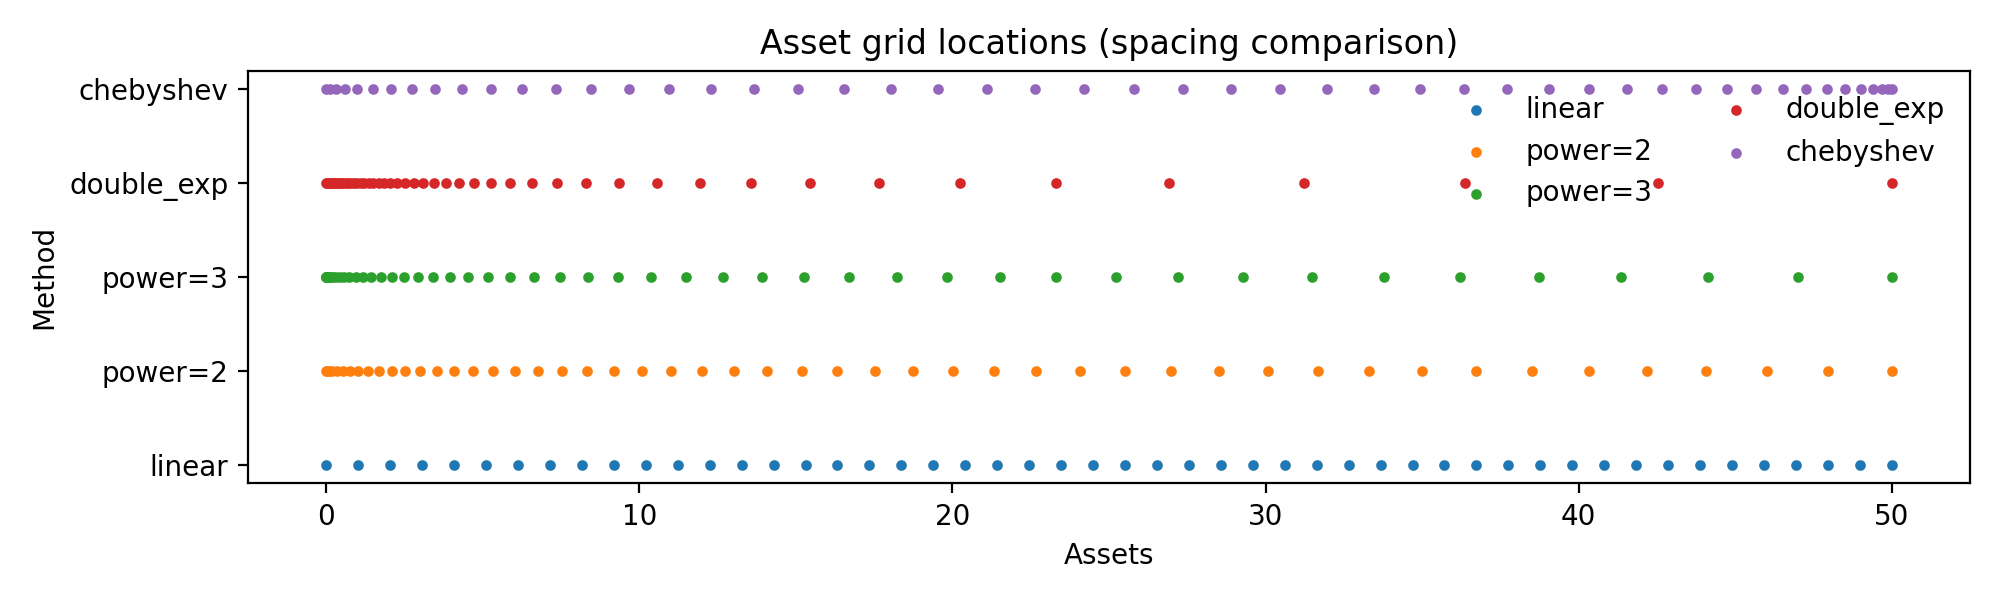
\includegraphics[width=0.95\textwidth]{figures/grids_asset_spacing.png}
    \caption{Asset grid spacing comparison: linear, power, double-exponential, and Chebyshev.}
\end{figure}

\begin{figure}[ht]
    \centering
    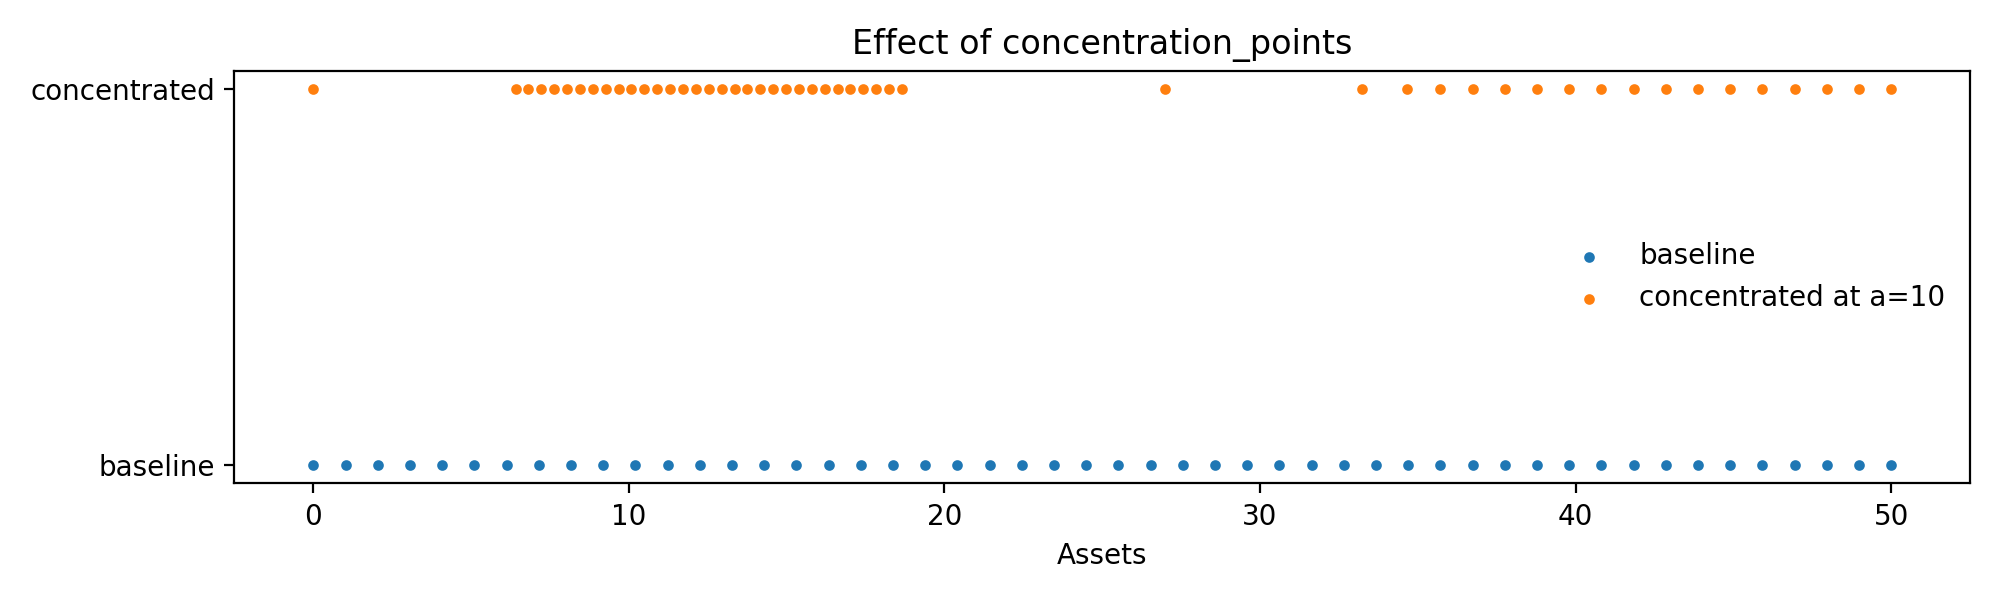
\includegraphics[width=0.95\textwidth]{figures/grids_concentration.png}
    \caption{Concentrated grid points around a kink at $a=10$ using \texttt{concentration\_points}.}
\end{figure}

\begin{figure}[ht]
    \centering
    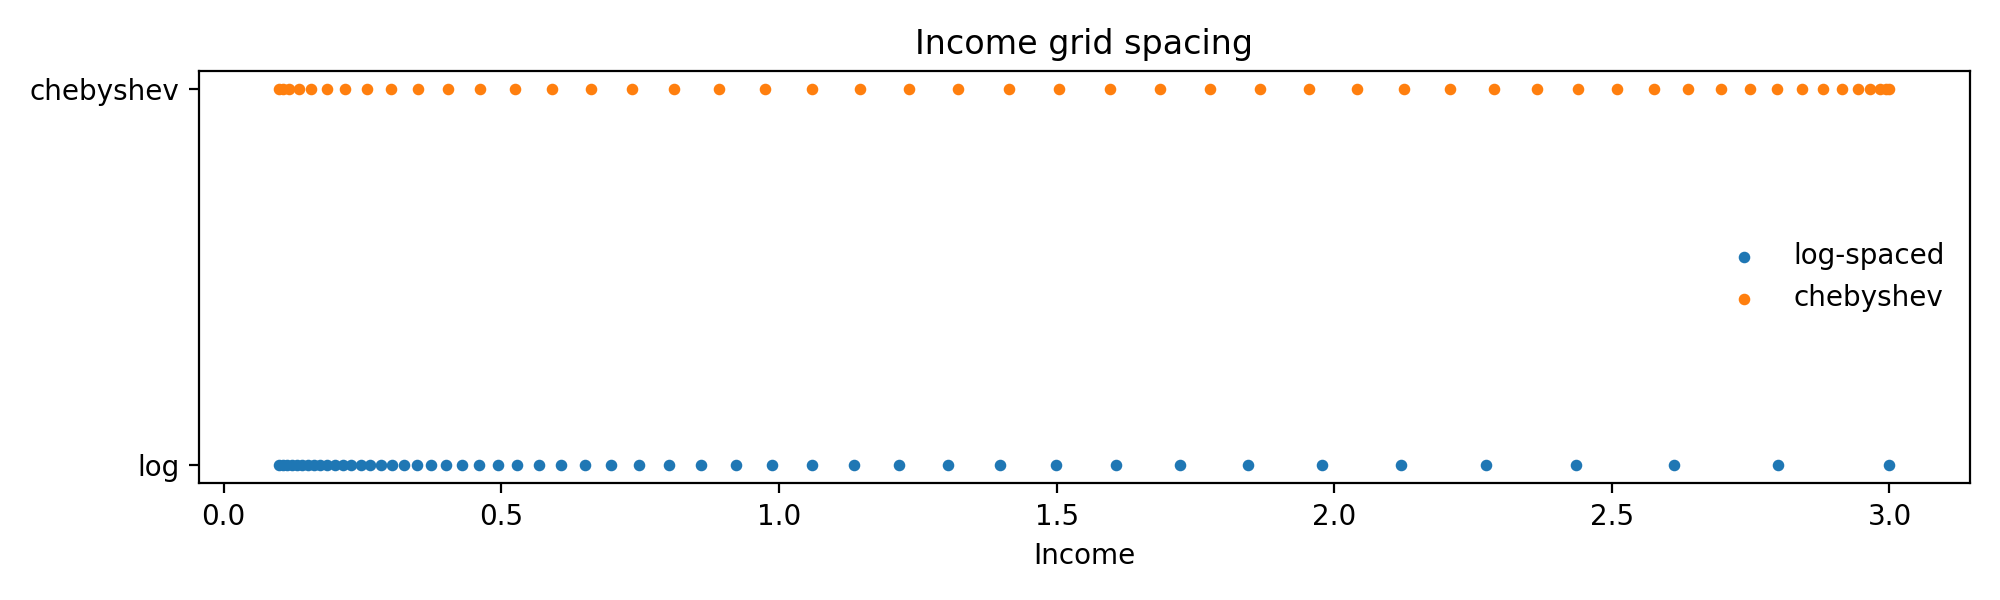
\includegraphics[width=0.95\textwidth]{figures/grids_income_spacing.png}
    \caption{Income grid spacing: log-spaced vs Chebyshev nodes on a bounded interval.}
\end{figure}

\begin{figure}[ht]
    \centering
    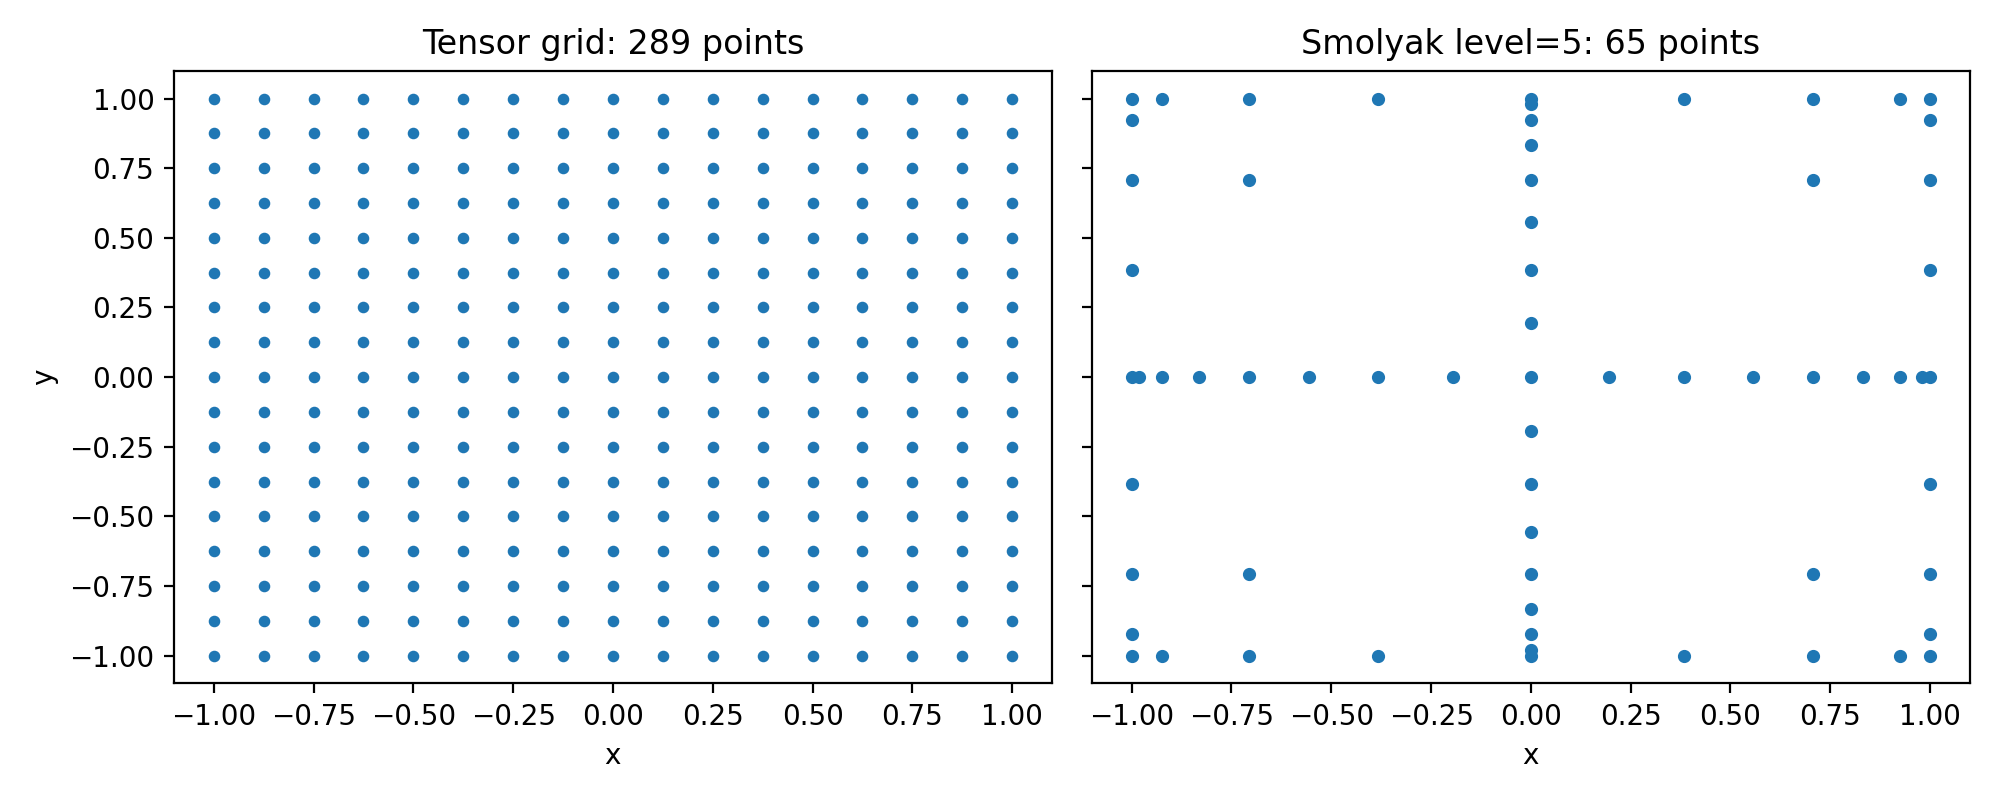
\includegraphics[width=0.95\textwidth]{figures/grids_tensor_vs_smolyak.png}
    \caption{Tensor product vs Smolyak sparse grid (2D), highlighting point-count reduction.}
\end{figure}

\subsection{\texttt{quadrature.py}}

\textbf{Purpose:} This section validates the quadrature functions with visual tests showing node placement, weight distribution, and accuracy. The examples are generated in the notebook:
\texttt{hetmacro/notebooks/test\_quadrature.ipynb}.

\noindent \textbf{Notebook reference:}
\begin{lstlisting}
# Notebook used to generate figures
hetmacro/notebooks/test_quadrature.ipynb
\end{lstlisting}

\noindent \textbf{Results:} Figure~\ref{fig:quadrature} displays all quadrature rules in a single panel. Each subplot shows nodes (circles, size proportional to weight) superimposed on the relevant function or PDF. The numerical tests in the notebook verify that all approximations match analytical values to high precision.

\begin{figure}[ht]
    \centering
    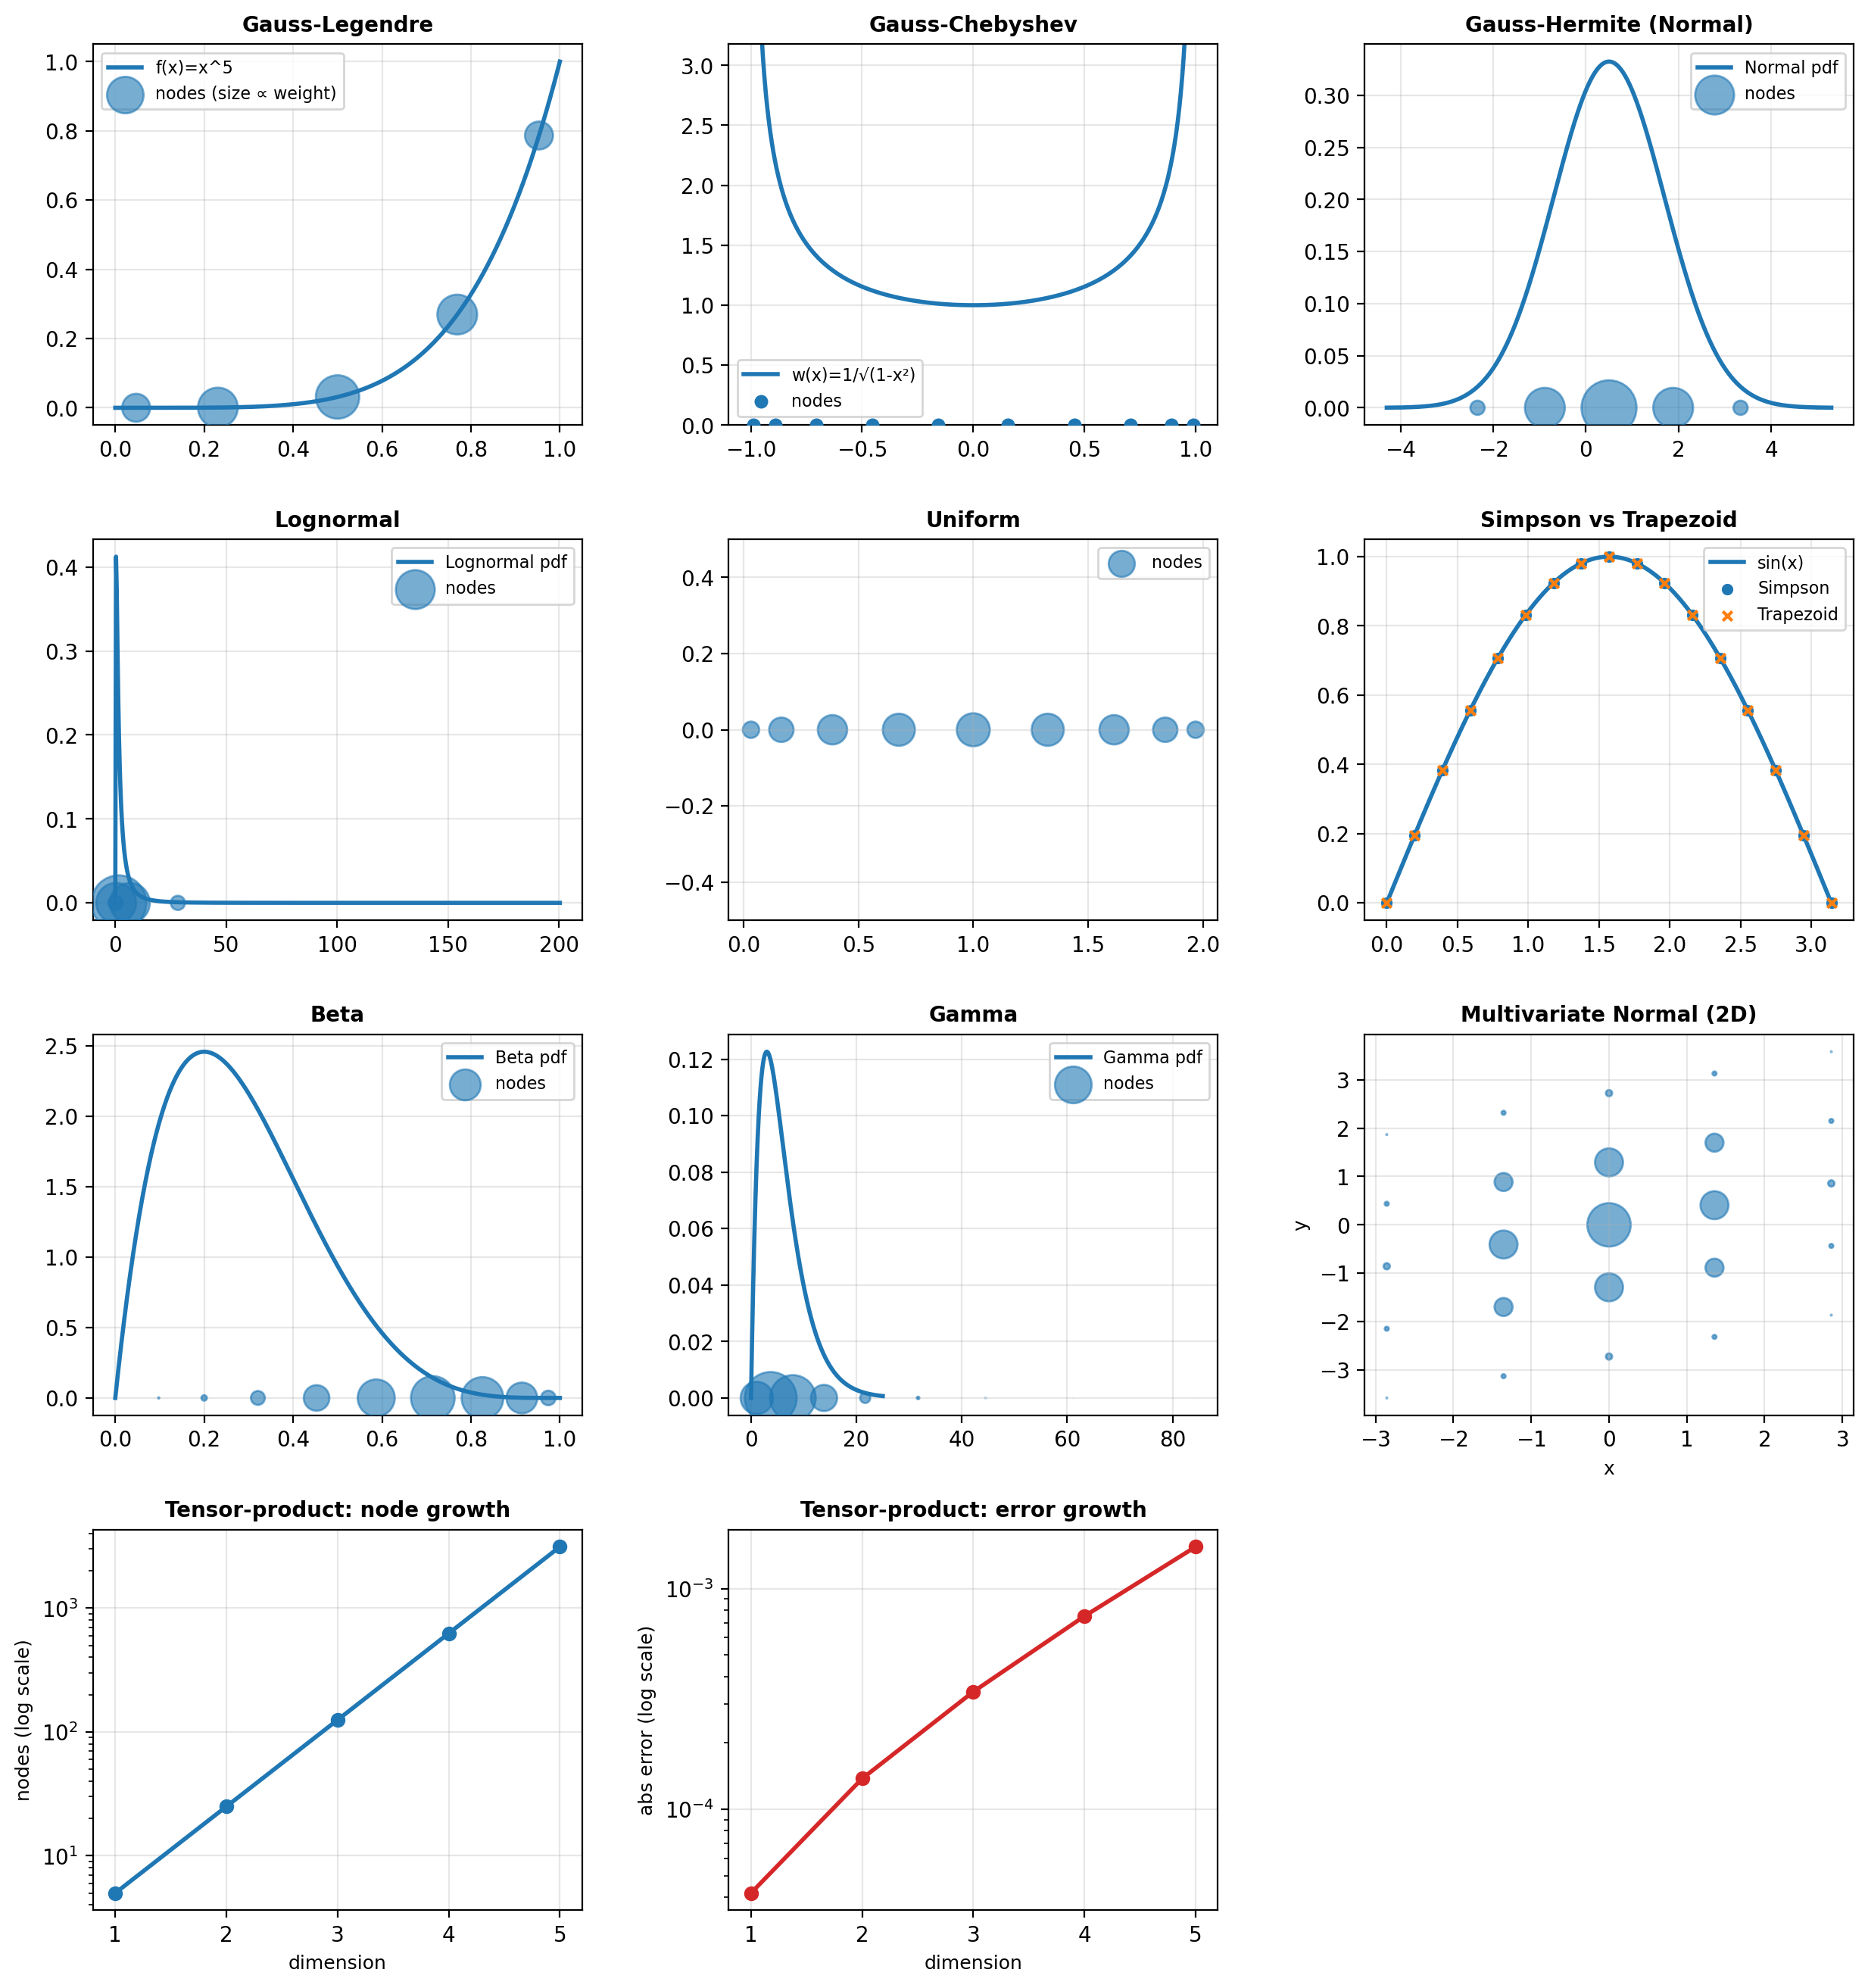
\includegraphics[width=0.95\textwidth]{figures/quadrature_visual_verification.png}
    \caption{Quadrature rules: visual verification of node placement and weights.}
    \label{fig:quadrature}
\end{figure}

\noindent \textbf{Subplot explanation:}

\begin{description}[style=nextline,leftmargin=1.5em]
    \item[Row 1 -- Gaussian quadrature (bounded and unbounded intervals)]
    \begin{itemize}
        \item \textbf{Gauss-Legendre:} Nodes for \texttt{qnwlege} on $[0,1]$ integrating $f(x)=x^5$. Nodes spread across the interval with weights (circle sizes) roughly uniform---optimal for smooth functions on bounded domains.
        \item \textbf{Gauss-Chebyshev:} Nodes for \texttt{qnwcheb} shown with the weight function $w(x)=1/\sqrt{1-x^2}$. Nodes cluster near endpoints where the weight function diverges---these are the Chebyshev points, optimal for polynomial interpolation.
        \item \textbf{Gauss-Hermite (Normal):} Nodes for \texttt{qnwnorm} overlaid on a normal PDF. Nodes cluster around the mean where probability mass concentrates, with larger weights (bigger circles) near the center.
    \end{itemize}

    \item[Row 2 -- Distribution-specific rules]
    \begin{itemize}
        \item \textbf{Lognormal:} Nodes for \texttt{qnwlogn} on the lognormal PDF. These are exponentiated Hermite nodes, naturally clustering where the skewed distribution has most mass.
        \item \textbf{Uniform:} Nodes for \texttt{qnwunif} on $[0,2]$. This is Legendre quadrature with weights normalized to sum to 1 (a probability distribution).
        \item \textbf{Simpson vs Trapezoid:} Newton-Cotes rules (\texttt{qnwsimp}, \texttt{qnwtrap}) for $\int_0^\pi \sin(x)\,dx = 2$. Both use equally-spaced nodes, but Simpson achieves higher accuracy through cubic interpolation.
    \end{itemize}

    \item[Row 3 -- Beta, Gamma, and multivariate normal]
    \begin{itemize}
        \item \textbf{Beta:} Nodes for \texttt{qnwbeta} with Beta$(2,5)$ PDF. Gauss-Jacobi nodes concentrate where the asymmetric Beta density peaks.
        \item \textbf{Gamma:} Nodes for \texttt{qnwgamma} with Gamma$(2,3)$ PDF. Gauss-Laguerre nodes cover the positive support, clustering near the mode.
        \item \textbf{Multivariate Normal (2D):} Tensor-product nodes from \texttt{qnwnorm\_mv} for a bivariate normal with correlation $\rho=0.3$. The elliptical pattern reflects the covariance structure; larger circles indicate higher-weight nodes near the mean.
    \end{itemize}

    \item[Row 4 -- Curse of dimensionality]
    \begin{itemize}
        \item \textbf{Node growth:} Total number of tensor-product nodes grows exponentially: $n^d$ for $n$ nodes per dimension in $d$ dimensions. With $n=5$, we have 5, 25, 125, 625, 3125 nodes for $d=1,\ldots,5$.
        \item \textbf{Error growth:} Despite exponentially more nodes, approximation error for $\mathbb{E}[\exp(\sum_i x_i)]$ under standard normal increases with dimension, illustrating the fundamental challenge of high-dimensional integration.
    \end{itemize}
\end{description}

% ==================================================================
\chapter{Heterogeneous Agent Tools}
% ==================================================================

% ------------------------------------------------------------------
\section{\texttt{backward.py} -- Dynamic Programming Solvers}
% ------------------------------------------------------------------

\subsection{Introduction and Economic Motivation}

The core of heterogeneous agent models is solving the household's Bellman equation:
\[
V(a, e) = \max_{c, a'} \left\{ u(c) + \beta \mathbb{E}[V(a', e') \mid e] \right\}
\]
subject to the budget constraint $c + a' = y(e) + (1+r)a$ and borrowing limit $a' \geq \underline{a}$.

Two main solution methods exist:
\begin{enumerate}
    \item \textbf{Value Function Iteration (VFI)}: Iterate on $V$ directly. Simple but slow.
    \item \textbf{Endogenous Grid Method (EGM)}: Iterate on marginal value $V_a$. Much faster because it exploits the first-order condition to avoid numerical optimization.
\end{enumerate}

\subsection{Function: \texttt{backward\_egm}}

\begin{lstlisting}
def backward_egm(
    Va: np.ndarray,
    Pi: np.ndarray,
    a_grid: np.ndarray,
    y: np.ndarray,
    r: float,
    beta: float,
    eis: float,
) -> Tuple[np.ndarray, np.ndarray, np.ndarray]
\end{lstlisting}

\textbf{Purpose:} Single backward step using the Endogenous Grid Method. Given tomorrow's marginal value $V_a'$, compute today's policies.

\textbf{Algorithm:}
\begin{enumerate}
    \item Compute expected marginal value: $W_a = \beta \Pi V_a'$
    \item Invert FOC to get consumption on endogenous grid: $c_{\text{endog}} = W_a^{-\text{eis}}$
    \item For each income state, interpolate to get policy on exogenous asset grid
    \item Apply borrowing constraint; update marginal value
\end{enumerate}

\textbf{Arguments:}
\begin{arglist}
    \item[\texttt{Va}] Marginal value of assets, shape \texttt{(n\_e, n\_a)}.
    \item[\texttt{Pi}] Income transition matrix, shape \texttt{(n\_e, n\_e)}.
    \item[\texttt{a\_grid}] Asset grid, shape \texttt{(n\_a,)}.
    \item[\texttt{y}] Income levels for each state, shape \texttt{(n\_e,)}.
    \item[\texttt{r}] Interest rate.
    \item[\texttt{beta}] Discount factor.
    \item[\texttt{eis}] Elasticity of intertemporal substitution ($= 1/\gamma$ for CRRA).
\end{arglist}

\returns{Tuple \texttt{(Va\_new, a\_policy, c\_policy)} of updated marginal value and policy functions.}

\connection{Called iteratively by \texttt{policy\_iteration}. Policies feed into \texttt{forward.py} for distribution iteration.}

\textbf{Example:}
\begin{lstlisting}
from hetmacro.backward import backward_egm
import numpy as np

# Initial guess: consume everything
n_e, n_a = 7, 200
coh = y[:, np.newaxis] + (1 + r) * a_grid[np.newaxis, :]
Va_init = (1 + r) * (0.05 * coh) ** (-1/eis)

# One EGM step
Va_new, a_pol, c_pol = backward_egm(
    Va_init, Pi, a_grid, y, r=0.02, beta=0.96, eis=1.0
)
\end{lstlisting}

\subsection{Function: \texttt{backward\_vfi}}

\begin{lstlisting}
def backward_vfi(
    V: np.ndarray,
    Pi: np.ndarray,
    a_grid: np.ndarray,
    y: np.ndarray,
    r: float,
    beta: float,
    gamma: float,
) -> Tuple[np.ndarray, np.ndarray, np.ndarray]
\end{lstlisting}

\textbf{Purpose:} Single VFI backward step with discrete choice over $a'$ in the grid. Slower than EGM but more general (works with non-differentiable preferences).

\textbf{Arguments:} Similar to \texttt{backward\_egm}, but uses \texttt{gamma} (risk aversion) instead of \texttt{eis}.

\returns{Tuple \texttt{(V\_new, a\_policy, c\_policy)}.}

\subsection{Function: \texttt{policy\_iteration}}

\begin{lstlisting}
def policy_iteration(
    Pi: np.ndarray,
    a_grid: np.ndarray,
    y: np.ndarray,
    r: float,
    beta: float,
    eis: float,
    method: str = "egm",
    tol: float = 1e-9,
    max_iter: int = 10000,
) -> Tuple[np.ndarray, np.ndarray, np.ndarray]
\end{lstlisting}

\textbf{Purpose:} Iterate backward steps until policy functions converge.

\textbf{Arguments:}
\begin{arglist}
    \item[\texttt{method}] Either \texttt{"egm"} or \texttt{"vfi"}.
    \item[\texttt{tol}] Convergence tolerance on policy function.
    \item[\texttt{max\_iter}] Maximum iterations.
\end{arglist}

\returns{Converged \texttt{(Va, a\_policy, c\_policy)}.}

\connection{Main entry point for solving household problem. Output is used by \texttt{forward.py} and \texttt{steady\_state.py}.}

% ------------------------------------------------------------------
\section{\texttt{forward.py} -- Distribution Iteration}
% ------------------------------------------------------------------

\subsection{Introduction and Economic Motivation}

Given optimal policies, we need the \emph{distribution} of agents across states to compute aggregates:
\[
A = \int a \, dD(a, e), \quad C = \int c(a, e) \, dD(a, e)
\]

The stationary distribution $D^*$ satisfies a fixed-point condition: if agents follow policy $a'(a, e)$ and income transitions according to $\Pi$, then $D^*$ is invariant.

\subsection{Function: \texttt{forward\_iteration}}

\begin{lstlisting}
def forward_iteration(
    D: np.ndarray, 
    Pi: np.ndarray, 
    a_i: np.ndarray, 
    a_pi: np.ndarray
) -> np.ndarray
\end{lstlisting}

\textbf{Purpose:} Single forward step for distribution. Given current distribution $D$, compute next period's distribution after agents save according to policy and income transitions.

\textbf{Arguments:}
\begin{arglist}
    \item[\texttt{D}] Current distribution, shape \texttt{(n\_e, n\_a)}.
    \item[\texttt{Pi}] Income transition matrix.
    \item[\texttt{a\_i}] Lottery lower indices from \texttt{get\_lottery}.
    \item[\texttt{a\_pi}] Lottery probabilities from \texttt{get\_lottery}.
\end{arglist}

\returns{Next period's distribution, same shape as \texttt{D}.}

\connection{Uses output of \texttt{get\_lottery} from \texttt{interpolation.py}.}

\subsection{Function: \texttt{stationary\_distribution}}

\begin{lstlisting}
def stationary_distribution(
    Pi: np.ndarray,
    a_policy: np.ndarray,
    a_grid: np.ndarray,
    tol: float = 1e-10,
    max_iter: int = 10000,
) -> np.ndarray
\end{lstlisting}

\textbf{Purpose:} Compute stationary distribution by iterating \texttt{forward\_iteration} until convergence.

\textbf{Arguments:}
\begin{arglist}
    \item[\texttt{Pi}] Income transition matrix.
    \item[\texttt{a\_policy}] Asset policy function, shape \texttt{(n\_e, n\_a)}.
    \item[\texttt{a\_grid}] Asset grid.
    \item[\texttt{tol}] Convergence tolerance.
    \item[\texttt{max\_iter}] Maximum iterations.
\end{arglist}

\returns{Stationary distribution $D^*$, shape \texttt{(n\_e, n\_a)}, summing to 1.}

\connection{Called by \texttt{household\_steady\_state} in \texttt{steady\_state.py}.}

\subsection{Functions: \texttt{expectation\_iteration}, \texttt{expectation\_functions}}

\begin{lstlisting}
def expectation_iteration(X, Pi, a_i, a_pi) -> np.ndarray
def expectation_functions(X, Pi, a_i, a_pi, T) -> np.ndarray
\end{lstlisting}

\textbf{Purpose:} Backward expectation operators for sequence-space Jacobian computation. Used internally by \texttt{ssj.py}.

% ------------------------------------------------------------------
\section{\texttt{steady\_state.py} -- Equilibrium Solvers}
% ------------------------------------------------------------------

\subsection{Introduction}

Heterogeneous agent models require market clearing. In the Aiyagari model:
\[
\underbrace{\int a \, dD(a, e; r)}_{\text{Asset supply } A(r)} = \underbrace{K(r)}_{\text{Capital demand}}
\]
We solve for the equilibrium interest rate $r^*$ that clears the asset market.

\subsection{Function: \texttt{household\_steady\_state}}

\begin{lstlisting}
def household_steady_state(
    Pi: np.ndarray,
    a_grid: np.ndarray,
    y: np.ndarray,
    r: float,
    beta: float,
    eis: float,
    method: str = "egm",
    tol: float = 1e-9,
) -> Dict[str, np.ndarray]
\end{lstlisting}

\textbf{Purpose:} Solve for household policies and distribution \emph{given} prices. This is the ``partial equilibrium'' household block.

\textbf{Arguments:}
\begin{arglist}
    \item[\texttt{Pi, a\_grid, y, r, beta, eis}] Model parameters.
    \item[\texttt{method}] Solution method (\texttt{"egm"} or \texttt{"vfi"}).
    \item[\texttt{tol}] Convergence tolerance.
\end{arglist}

\returns{Dictionary containing:}
\begin{itemize}
    \item \texttt{"D"}: Stationary distribution
    \item \texttt{"Va"}: Marginal value function
    \item \texttt{"a"}, \texttt{"c"}: Policy functions
    \item \texttt{"a\_i"}, \texttt{"a\_pi"}: Lottery indices/weights
    \item \texttt{"A"}, \texttt{"C"}: Aggregate asset holdings and consumption
    \item All input parameters
\end{itemize}

\connection{Called repeatedly by \texttt{market\_clearing} at different interest rates.}

\subsection{Function: \texttt{market\_clearing}}

\begin{lstlisting}
def market_clearing(
    r_bounds: Tuple[float, float],
    household_ss_func: Callable[[float], Dict],
    K_demand_func: Callable[[float], float],
    tol: float = 1e-6,
    max_iter: int = 100,
) -> Dict[str, np.ndarray]
\end{lstlisting}

\textbf{Purpose:} Find equilibrium interest rate using bisection on excess demand.

\textbf{Arguments:}
\begin{arglist}
    \item[\texttt{r\_bounds}] Tuple \texttt{(r\_low, r\_high)} bracketing equilibrium rate.
    \item[\texttt{household\_ss\_func}] Function mapping $r \mapsto$ household steady state dict.
    \item[\texttt{K\_demand\_func}] Function mapping $r \mapsto$ capital demand.
    \item[\texttt{tol}] Tolerance on excess demand.
    \item[\texttt{max\_iter}] Maximum bisection iterations.
\end{arglist}

\returns{Household steady state dict at equilibrium $r^*$.}

\textbf{Example:}
\begin{lstlisting}
from hetmacro.steady_state import market_clearing

def hh_ss(r):
    y = w * np.exp(e)  # wage * productivity
    return household_steady_state(Pi, a_grid, y, r, beta, eis)

def K_demand(r):
    return (alpha / (r + delta)) ** (1/(1-alpha))

ss = market_clearing(
    r_bounds=(0.005, 0.04),
    household_ss_func=hh_ss,
    K_demand_func=K_demand
)
print(f"Equilibrium r = {ss['r']:.4f}")
\end{lstlisting}

% ------------------------------------------------------------------
\section{\texttt{ssj.py} -- Sequence-Space Jacobians}
% ------------------------------------------------------------------

\subsection{Introduction and Economic Motivation}

For aggregate dynamics (impulse responses, business cycle analysis), we need to know how aggregates respond to shocks. The \textbf{sequence-space Jacobian} $\mathcal{J}$ captures:
\[
\begin{pmatrix} dA_0 \\ dA_1 \\ \vdots \\ dA_{T-1} \end{pmatrix} = \mathcal{J} \begin{pmatrix} dr_0 \\ dr_1 \\ \vdots \\ dr_{T-1} \end{pmatrix}
\]

The ``fake news algorithm'' (Auclert et al., 2021) efficiently computes these Jacobians by exploiting the structure of the household problem.

\subsection{Function: \texttt{jacobian}}

\begin{lstlisting}
def jacobian(
    ss: Dict[str, np.ndarray], 
    shocks: Dict[str, Dict[str, float]], 
    T: int
) -> Dict[str, Dict[str, np.ndarray]]
\end{lstlisting}

\textbf{Purpose:} Compute Jacobians of aggregate outputs (A, C) with respect to input shocks.

\textbf{Arguments:}
\begin{arglist}
    \item[\texttt{ss}] Steady state dict from \texttt{household\_steady\_state}.
    \item[\texttt{shocks}] Dict mapping shock names to input perturbations. E.g., \texttt{\{"r": \{"r": 1.0\}\}} for interest rate shock.
    \item[\texttt{T}] Horizon length.
\end{arglist}

\returns{Nested dict: \texttt{Js["A"]["r"]} is the $T \times T$ Jacobian of assets w.r.t. interest rate.}

\textbf{Example:}
\begin{lstlisting}
from hetmacro.ssj import jacobian

# Compute Jacobian at steady state
shocks = {"r": {"r": 1.0}}  # unit shock to r
T = 300
Js = jacobian(ss, shocks, T)

# Impulse response of assets to 1% interest rate shock
dA = Js["A"]["r"] @ (0.01 * np.ones(T))
\end{lstlisting}

\subsection{Function: \texttt{step1\_backward}}

\begin{lstlisting}
def step1_backward(
    ss: Dict,
    shock: Dict[str, float],
    T: int,
    h: float = 1e-4,
) -> Tuple[Dict[str, np.ndarray], np.ndarray]
\end{lstlisting}

\textbf{Purpose:} Step 1 of fake news algorithm: compute ``curlyY'' (direct effect) and ``curlyD'' (distribution response).

\subsection{Function: \texttt{J\_from\_F}}

\begin{lstlisting}
def J_from_F(F: np.ndarray) -> np.ndarray
\end{lstlisting}

\textbf{Purpose:} Convert fake news matrix $F$ to Jacobian $J$ via cumulative summation.

% ==================================================================
\chapter{Example: Aiyagari Model}
% ==================================================================

\section{\texttt{models/aiyagari.py}}

This module demonstrates how to combine \texttt{hetmacro} tools to solve a complete model.

\subsection{Function: \texttt{solve\_steady\_state}}

\begin{lstlisting}
def solve_steady_state(
    beta: float = 0.96,
    eis: float = 1.0,
    rho: float = 0.9,
    sigma: float = 0.2,
    n_e: int = 7,
    amin: float = 0.0,
    amax: float = 50.0,
    n_a: int = 500,
    alpha: float = 0.36,
    delta: float = 0.08,
    r_bounds: Tuple[float, float] = (0.005, 0.04),
) -> Dict[str, np.ndarray]
\end{lstlisting}

\textbf{Purpose:} Solve the Aiyagari model steady state with idiosyncratic income risk.

\textbf{Workflow:}
\begin{enumerate}
    \item Discretize income process using \texttt{rouwenhorst}
    \item Create asset grid using \texttt{make\_asset\_grid}
    \item Define household problem given prices
    \item Find market-clearing interest rate using \texttt{market\_clearing}
\end{enumerate}

\textbf{Example:}
\begin{lstlisting}
from hetmacro.models.aiyagari import solve_steady_state
import matplotlib.pyplot as plt

# Solve model
ss = solve_steady_state(
    beta=0.96, 
    eis=1.0, 
    rho=0.9, 
    sigma=0.2,
    n_a=500
)

print(f"Equilibrium interest rate: {ss['r']:.4f}")
print(f"Aggregate capital: {ss['K']:.2f}")
print(f"Aggregate consumption: {ss['C']:.2f}")

# Plot consumption policy
plt.figure(figsize=(10, 6))
for i in range(ss['c'].shape[0]):
    plt.plot(ss['a_grid'], ss['c'][i], label=f'e={i}')
plt.xlabel('Assets')
plt.ylabel('Consumption')
plt.title('Consumption Policy Functions')
plt.legend()
plt.show()
\end{lstlisting}

\end{onehalfspacing}

% ==================================================================
\chapter{Quick Reference}
% ==================================================================

\section{Module Dependency Graph}

\begin{verbatim}
                    +----------+
                    |  grids   |
                    +----+-----+
                         |
         +---------------+---------------+
         |               |               |
    +----v----+    +-----v-----+    +----v----+
    |quadrature|    |interpolation|    | markov |
    +---------+    +-----+-----+    +----+----+
                         |               |
                         +-------+-------+
                                 |
                    +------------v-----------+
                    |       backward         |
                    +------------+-----------+
                                 |
                    +------------v-----------+
                    |        forward         |
                    +------------+-----------+
                                 |
              +-----------------+------------------+
              |                                    |
    +---------v---------+              +-----------v-----------+
    |   steady_state    |              |         ssj           |
    +-------------------+              +-----------------------+
\end{verbatim}

\section{Common Workflows}

\subsection{Solving a Steady State}
\begin{lstlisting}
from hetmacro.grids import make_asset_grid
from hetmacro.markov import rouwenhorst
from hetmacro.steady_state import household_steady_state, market_clearing

# 1. Set up grids and income process
a_grid = make_asset_grid(0, 50, 500)
e, Pi = rouwenhorst(7, rho=0.95, sigma=0.1)

# 2. Define household problem
def hh_ss(r):
    y = w(r) * np.exp(e)
    return household_steady_state(Pi, a_grid, y, r, beta, eis)

# 3. Find equilibrium
ss = market_clearing((0.01, 0.04), hh_ss, K_demand)
\end{lstlisting}

\subsection{Computing Impulse Responses}
\begin{lstlisting}
from hetmacro.ssj import jacobian

# 1. Get steady state
ss = solve_steady_state(...)

# 2. Compute Jacobians
Js = jacobian(ss, {"r": {"r": 1.0}}, T=300)

# 3. Construct impulse response
shock_path = np.zeros(300)
shock_path[0] = 0.01  # 1% shock at t=0
dA = Js["A"]["r"] @ shock_path
\end{lstlisting}

\end{document}
